\documentclass{article}
\usepackage{pgfplots}
\usepackage[utf8]{inputenc}
\begin{document}
\begin{center}
	\begin{tikzpicture}
	\begin{axis}[
	ylabel=gyakoriság,
	enlarge x limits=4,
	legend style={
	    at={(0.5,-0.15)},
	    anchor=north,legend columns=-1
	},
	ymin=0,
	ymax=16,
	ybar,
	xtick=data,
	symbolic x coords={lany, fiu},
	grid=major,
	xmajorgrids=false
	]
	\addplot coordinates {(lany,0)(fiu,0)};
	%\legend{0-10,10-20,20-30,$>30$}
	\end{axis}
	\end{tikzpicture}	
		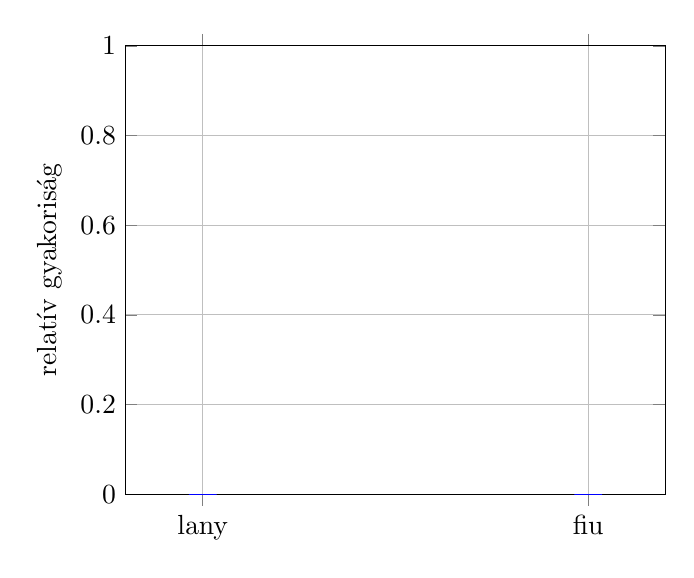
\begin{tikzpicture}
		\begin{axis}[
		ylabel=relatív gyakoriság,
		enlarge x limits=0.2,
		legend style={
		    at={(0.5,-0.15)},
		    anchor=north,legend columns=-1
		},
		ymin=0,
		ymax=1,
		ybar,
		xtick=data,
		symbolic x coords={lany, fiu},
		grid=major,
		xmajorgrids=true
		]
		\addplot coordinates {(lany,0) (fiu,0)};
		%\legend{0-10,10-20,20-30,$>30$}
		\end{axis}
		\end{tikzpicture}
		
	
\end{center}


\begin{tikzpicture}
\begin{axis}[
    ybar,
    enlargelimits=0.4,
    symbolic x coords={A,B},
    xtick=data,
    ymin=0,
    nodes near coords,
    bar shift=0pt
    ]
\addplot coordinates {(A,0)(B,0)};
\addplot coordinates {(B,0)};
\end{axis}
\end{tikzpicture}

\end{document}